\begin{frame}
    \begin{exampleblock}{Exercise V}
        \begin{enumerate}
            \item Get the Arduino\textregistered{} \acs{ide} of your choice.
            \item Connect the board to your \acs{pc}.
            \item Connect the board, push button, \acs{led} and resistor.
            \item When the push button is pressed:
                  \begin{enumerate}
                      \item Turn the \acs{led} on.
                      \item Click or press the \key{Left Mouse Button}.
                      \item Log a message to the serial terminal.
                  \end{enumerate}
            \item When the push button is released:
                  \begin{enumerate}
                      \item Turn the \acs{led} off.
                  \end{enumerate}
        \end{enumerate}
        \par Hint:
        \begin{itemize}
            \item \href{https://docs.arduino.cc/tutorials/nano-rp2040-connect/rp2040-01-technical-reference\#usb-keyboard}{Arduino\textregistered{} Cheat Sheat - USB Keyboard}
            \item \href{https://github.com/arduino/ArduinoCore-mbed/tree/main/libraries/USBHID}{\acs{usb}\acs{hid} Library}
        \end{itemize}
    \end{exampleblock}
\end{frame}

\begin{frame}{Solution: Exercise V}
    \begin{listing}[H]
        \inputsource[fontsize=\fontsize{10}{10}]{c}{arduino/usb_mouse_click_pullup.c}
        \caption{Solution for Exercise V (pin mode: \mintinline{c}{INPUT}).}
        \label{lst:arduino:exercise:5:solution:pullup}
    \end{listing}
\end{frame}

\begin{frame}{Solution: Exercise V}
    \begin{figure}
        \begin{tikzpicture}
            \ctikzset{bipoles/length=1cm, !vi/.style={no v symbols, no i symbols}, bipole voltage style/.style={text opacity=0}, bipole current style/.style={color=ttw-red}}
            \draw (2,4) node[rp2040] (rp20401) {}
            (rp20401.D2) to ++(4,0) to ++(0,4) to ++(1.5,0) to ++(0,-1) to [R,name=R1,l={$R_1 = \SI{220}{\ohm}$},v=$U_1$,voltage shift=4.5,!vi] ++(0,-1) to [leDo,name=LED,l=$D_1$,v=$U_2$,i=$i$,voltage shift=4.5,!vi] ++(0,-2)
            (rp20401.GNDR) to ++(5.5,0) to ++(0,0.5);
            \fixedvlen[0.5cm]{R1}{$U_1$}[tw-blue]
            \fixedvlen[0.5cm]{LED}{$U_2$}[tw-blue]
            \iarronly{LED}

            \draw (rp20401.D3) to ++(0.5, 0) to ++(0, 1.25) to ++(1,0) node[fill=black, circle, inner sep=0pt, minimum size=1mm] {};
            \draw (rp20401.D12) ++(1.5, -0.25) node[vcc] {\scriptsize\texttt{VIN}} to ++(0, -0.25) to [R,name=R2,l={$R_2 = \SI{10}{\kilo\ohm}$},v=$U_3$,voltage shift=4.5,!vi] ++(0, -1.5) to [nopb, name=PB, l=$S_1$] ++(0, -1.25) node[rground] {};
            \fixedvlen[0.5cm]{R2}{$U_3$}[tw-blue]
        \end{tikzpicture}
        \caption{Circuit for Exercise V (pin mode: \mintinline{c}{INPUT})}
    \end{figure}
\end{frame}

\begin{frame}{Solution: Exercise V}
    \begin{listing}[H]
        \inputsource[fontsize=\fontsize{8}{8}]{c}{arduino/usb_mouse_click.c}
        \caption{Solution for Exercise V (pin mode: \mintinline{c}{INPUT_PULLUP}).}
        \label{lst:arduino:exercise:5:solution:click}
    \end{listing}
\end{frame}

\begin{frame}{Solution: Exercise V}
    \begin{figure}
        \begin{tikzpicture}
            \ctikzset{bipoles/length=1cm, !vi/.style={no v symbols, no i symbols}, bipole voltage style/.style={text opacity=0}, bipole current style/.style={color=ttw-red}}
            \draw (2,4) node[rp2040] (rp20401) {}
            (rp20401.D2) to ++(4,0) to ++(0,4) to ++(1.5,0) to ++(0,-1) to [R,name=R1,l={$R_1 = \SI{220}{\ohm}$},v=$U_1$,voltage shift=4.5,!vi] ++(0,-1) to [leDo,name=LED,l=$D_1$,v=$U_2$,i=$i$,voltage shift=4.5,!vi] ++(0,-2)
            (rp20401.GNDR) to ++(5.5,0) to ++(0,0.5);
            \fixedvlen[0.5cm]{R1}{$U_1$}[tw-blue]
            \fixedvlen[0.5cm]{LED}{$U_2$}[tw-blue]
            \iarronly{LED}

            \draw (rp20401.D3) to ++(0.5, 0) to ++(0, 3.65) to ++(1,0) to [nopb, name=PB, l=$S_1$] ++(0, -3.5) node[rground] {};
        \end{tikzpicture}
        \caption{Circuit for Exercise V (pin mode: \mintinline{c}{INPUT_PULLUP})}
    \end{figure}
\end{frame}

\begin{frame}{Solution: Exercise V}
    \begin{figure}
        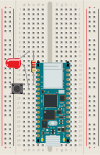
\includegraphics[width=0.35\textwidth]{images/microcontroller/exercises/exercise-5-solution.pdf}
        \caption{Solution for Exercise V.}
    \end{figure}
\end{frame}

\begin{frame}{Solution: Exercise V}
    \begin{figure}
        % https://learn.adafruit.com/assets/59149
        \includegraphics[width=0.9\textwidth]{images/microcontroller/actuators/switch_bounce.jpg}
        \caption{Bouncing of switches and push buttons.}
    \end{figure}
\end{frame}

\begin{frame}{Solution: Exercise V}
    \begin{listing}[H]
        \inputsource[fontsize=\fontsize{8}{8}]{c}{arduino/usb_mouse_press.c}
        \caption{Solution for Exercise V (press and release).}
        \label{lst:arduino:exercise:5:solution:press_release}
    \end{listing}
\end{frame}

\begin{frame}{Solution: Exercise V}
    \begin{listing}[H]
        \inputsource[fontsize=\fontsize{8}{8}, lastline=21]{c}{arduino/usb_mouse_click_debounce.c}
        \caption{Solution for Exercise V (click, debounced; \mintinline{c}{setup()}).}
        \label{lst:arduino:exercise:5:solution:click:debounce:setup}
    \end{listing}
\end{frame}

\begin{frame}{Solution: Exercise V}
    \begin{listing}[H]
        \inputsource[fontsize=\fontsize{8}{8}, firstline=23]{c}{arduino/usb_mouse_click_debounce.c}
        \caption{Solution for Exercise V (click, debounced; \mintinline{c}{loop()}).}
        \label{lst:arduino:exercise:5:solution:click:debounce:loop}
    \end{listing}
\end{frame}

\begin{frame}{Solution: Exercise V}
    \begin{listing}[H]
        \inputsource[fontsize=\fontsize{8}{8}, firstline=23]{c}{arduino/usb_mouse_press_debounce.c}
        \caption{Solution for Exercise V (press and release, debounced, \mintinline{c}{loop(c)}).}
        \label{lst:arduino:exercise:5:solution:press_release:debounce}
    \end{listing}
\end{frame}